\documentclass[showpacs, preprintnumbers, pra, superscriptaddress, floatfix, onecolumn, longbibliography]{revtex4-1}
\usepackage{amssymb}
\usepackage{amsmath}
\usepackage{float}
\usepackage{graphicx}
\usepackage{epsfig}
\usepackage[T1]{fontenc}
\usepackage{color}


\usepackage[utf8]{inputenc}
%\topmargin=0.2cm

\newcommand{\beq}{\begin{equation}}
\newcommand{\eeq}{\end{equation}}
\newcommand{\bea}{\begin{eqnarray}}
\newcommand{\eea}{\end{eqnarray}}
\newcommand{\nn}{\nonumber}
\newcommand{\no}{\noindent}
\newcommand{\hs}{\hspace{0.1cm}}
\newcommand{\spz}{\hspace{0.7cm}}
\newcommand{\st}{\stackrel}
\newcommand{\eps}{\epsilon}
\newcommand{\veps}{\varepsilon}
\newcommand{\al}{\alpha}
\newcommand{\s}{\sigma}
\newcommand{\lam}{\lambda}
\newcommand{\om}{\omega}
\newcommand{\iom}{i\omega_n}
\newcommand{\de}{\delta}
\newcommand{\D}{\Delta}
\newcommand{\goto}{\rightarrow}
\newcommand{\lab}{\label}
\newcommand{\be}{\beta}
\newcommand{\zb}{\bar{z}}
\newcommand{\p}{\partial}\newcommand{\vp}{\varphi}
\newcommand{\ra}{\rangle}
\newcommand{\la}{\langle}
\newcommand{\Ga}{\Gamma}
\newcommand{\ga}{\gamma}
\newcommand{\app}{\approx}
\newcommand{\ua}{\uparrow}
\newcommand{\da}{\downarrow}
\newcommand{\Ua}{\Uparrow}
\newcommand{\Da}{\Downarrow}
\newcommand{\dmi}{\frac{1}{2}}
\newcommand{\lra}{\longrightarrow}
\newcommand{\Lra}{\Leftrightarrow}
\newcommand{\tht}{\theta}
\newcommand{\pbf}{}
\newcommand{\SM}{S}
\newcommand{\uul}[1] {\underline{\underline{ #1}}}
\def\mean#1{\left< #1 \right>}

\begin{document}

\title{}


\maketitle

\section{DFT on MnBi$_2$Te$_4$}

\subsection{Methods}

To estimate parameters of the low-energy model, we performed  density-functional calculations (DFT) using as structural model a slab consisting of six MnBi$_2$Te$_4$ unit cells with a vacuum of 30 Bohr radiie (Fig. \ref{dft_structure}a)
We use the experimental bulk lattice parameters and atomic positions.
The calculations are based on the GGA+U method with the generalized grandient approximation \cite{perdew1996generalized} as implemented in the FPLO code version 48.00-52 \cite{PhysRevB.59.1743}. We fix parameters $U=5.34\,$eV and $J=0$, as in Ref. \cite{otrokov2019prediction} and use the atomic limit flavor for the double counting correction. The spin-orbit interaction is considered in the fully-relativistic four-component formalism. Numerial k-space integrations are performed with a tetrahedron method with a mesh of $12\times12\times1$ subdivisions in the Brillouin zone. For the calculations of the density of states (DOS), we consider a mesh of $36\times36\times3$ subdivisions.

\begin{figure*}[h!]
 \centering
 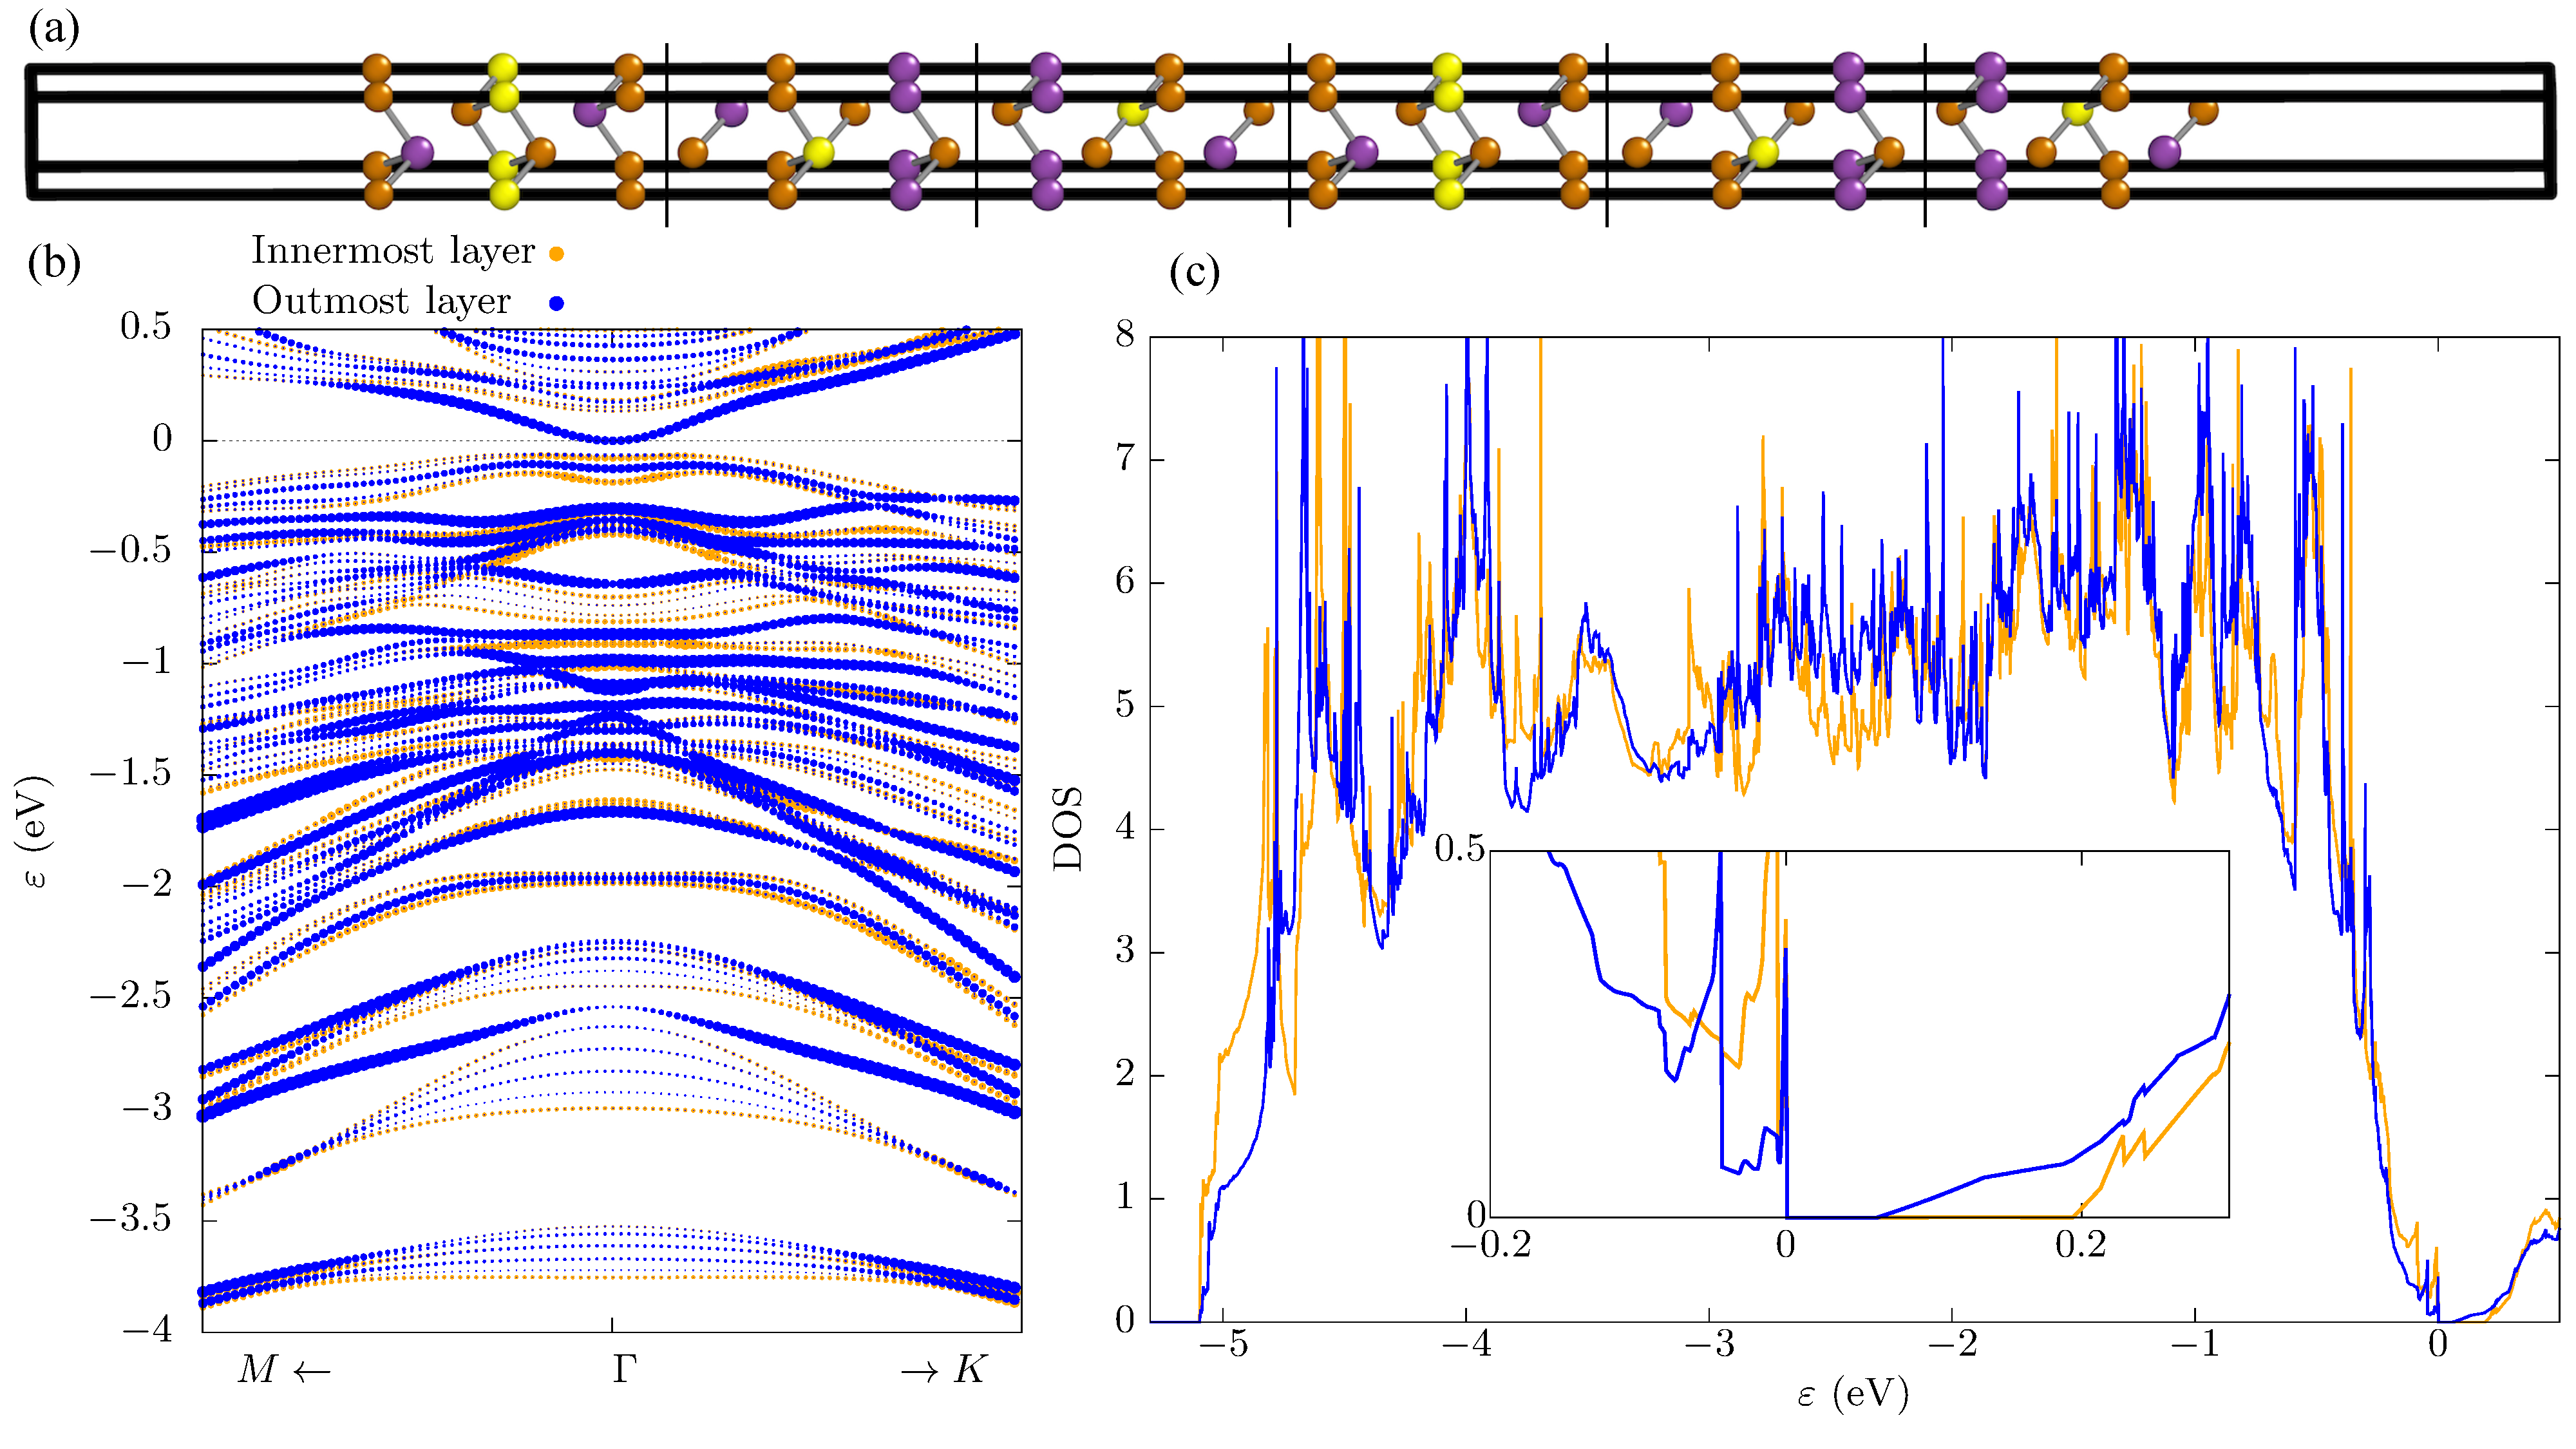
\includegraphics[width=18 cm]{plot.pdf}
	\caption{a) Structural model used in the density-functional calculation. b,c) Projection of the bandstructure and DOS, respectively, on the innermost and outermost layers of the slab.}
	\label{dft_structure}
\end{figure*}

\subsection{Estimation of parameters}

\subsubsection{Chemical potential}

\subsubsection{Mn - Mn in-plane exchange and magnetic anisotropy}
Regarding the magnetic anisotropy $K$, Ref. \cite{otrokov2019prediction} finds 0.225 meV per Mn atom, while we found 0.38 meV per Mn atom. \textcolor{red}{Check with Manuel}.

Regarding the in-plane exchange, Ref. \cite{otrokov2019prediction} finds 0.09 meV per $\mu_B$

\subsubsection{Surface density}

\subsubsection{Surface gap}

\subsubsection{Fermi velocity}




\bibliography{ref}
\end{document}


